% !TEX root = ../../buch.tex
% loesung.tex -- Beispiel-File für die Beschreibung der Loesung
%
% (c) 2020 Prof Dr Andreas Müller, Hochschule Rapperswil
%
\section{Lösungsmethoden
\label{burgers:section:loesung}}
\rhead{Lösungsmethoden}

Das \autoref{chapter:pde} beschreibt den theoretischen Aspekt der Numerik  partieller Differentialgleichungen.
In diesem Abschnitt wird auf die numerischen Lösungsmethoden der Gleichung von Burgers eingegangen.


\subsection{Explizit}

Bei der Lösung der Gleichung mit dem expliziten Ansatz werden für die Berechnung des gewünschten Punktes $u_i^n$, auf Gitterpunkte einen Zeitschritt in der Vergangenheit $u^{n-1}$ zurückgegriffen.
Nachfolgend werden zwei grundlegende Varianten mit jeweils einer kleinen Variation aufgezeigt.

\subsubsection{Lineare Methoden}

	Die Ableitung in der Zeit wird mit der Differenz der beiden Punkte $u_{i}^{n}-u_{i}^{n-1}$ realisiert.
	Die Ableitung im Raum wird mit der Differenz $u_{i}^{n-1}-u_{i-1}^{n-1}$ abstrahiert.
	Sie wird grafisch in \autoref{burgers:fig:Linear1} dargestellt.


	     \begin{figure}
		\centering
		\includegraphics[height=.4\textwidth]{papers/burgers/BurgersEquation/tikz/linear1/linear1.pdf}
		\caption{Lineare explizite Methode}
		\label{burgers:fig:Linear1}
		\end{figure}

	Die grundlegende Gleichung \eqref{burgers:eq_invisid_burgers} kann mit der gewählten Methode
	\begin{equation}
	  	\frac {\partial u}{\partial t}+u{\frac {\partial u}{\partial x}} \cong \frac{u_{i}^{n}-u_{i}^{n-1}}{\Delta t}+ u_{i}^{n}\, \frac{u_{i}^{n-1}-u_{i-1}^{n-1}}{\Delta x}=0
	  	  \label{burgers:eq_ex_lin1}
	  	\end{equation}
        umgeschrieben werden.
	  	Für die Lösung muss die Gleichung \eqref{burgers:eq_ex_lin1} nach

	  	\begin{equation}
	  u_{i}^{n} = \frac{\Delta{x}\, u^{n-1}_{i}\,}{- \Delta{t}\, u^{n-1}_{i-1}\, + \Delta{t}\, u^{n-1}_{i}\, + \Delta{x}\,}
		  \label{burgers:eq_ex_sol_lin1}
	\end{equation}
 	aufgelöst werden.

\medskip

	Für die Multiplikation des zweiten Bruches muss nicht unbedingt der gesuchte Punkt $u_{i}^{n}$ verwendet werden (Siehe dazu die grafische Darstellung in \autoref{burgers:fig:Linear2}).
	Es kann sowohl der Punkt auf gleicher Stelle im Raum, als auch einen Zeitschritt in der Vergangenheit verwendet werden.


     \begin{figure}
	\centering
	\includegraphics[height=.4\textwidth]{papers/burgers/BurgersEquation/tikz/linear2/linear2.pdf}
	\caption{Lineare explizite Methode mit  $u_{i}^{n-1}$ f\"ur die Multiplikation}
	\label{burgers:fig:Linear2}
	\end{figure}
	Die Gleichung
	\begin{equation}
			\frac {\partial u}{\partial t}+u{\frac {\partial u}{\partial x}} \cong \frac{u_{i}^{n}-u_{i}^{n-1}}{\Delta t}+ u_{i}^{n-1}\, \frac{u_{i}^{n-1}-u_{i-1}^{n-1}}{\Delta x}=0
		\label{burgers:eq_ex_lin2}
	\end{equation}
	ändert sich nur minimal.
	 Auch kann wieder eine Lösung für den Wert im Punkt

	\begin{equation}
		u_{i}^{n} = \frac{u^{n-1}_{i}\, \left(\Delta{t}\, u^{n-1}_{i-1}\, - \Delta{t}\, u^{n-1}_{i}\, + \Delta{x}\,\right)}{\Delta{x}\,}
    	\label{burgers:eq_ex_sol_lin2}
	\end{equation}
gefunden werden.

\subsubsection{Stabilit\"atskriterium lineare Methoden}
	Die Stabilit\"at kann f\"ur diese L\"osungsmethode nicht garantiert werden.
	Sie folgt dem Courant-Friedrichs-Lewy-Kriterium
\index{Courant-Friedrichs-Lewy-Kriterium}%
	\begin{equation}
		  c = \frac{u \, \Delta t}{\Delta x} < c_{\text{krit}}.
	\end{equation}
	$ \Delta t$ und $\Delta x$  beschreiben die diskrete Schrittgr\"osse.
	Das Kriterium $c_{\text{krit}}$ ist von der gew\"ahlten L\"osungsmethode abh\"anig.
	Beim expliziten Verfahren beträgt $c_{\text{krit}} = 1$.
	Falls $c_{\text{krit}} > 1$ bedeutet dies, dass das Verh\"altnis zwischen $ \Delta t$ und $\Delta x$ zu gross ist und die Berechnungen instabil werden.
	F\"ur diesen Fall und mit der Annahme $u = 1$ m\"usste $ \Delta t$ gr\"osser sein als $\Delta x$.
	Dies macht intuitiv Sinn, da der Raum nicht feiner abgetastet werden sollte als die Zeit.



\subsubsection{Leap-Frog Methode}
\index{Leap-Frog Methode}%
	Bei genauer Betrachtung der Ableitungen in \autoref{burgers:fig:Linear1} und \autoref{burgers:fig:Linear2} erkennt man, dass sich die berechnete Ableitung eigentlich zwischen den beiden Punkten befindet.
	Grunds\"atzlich sollte man für ein optimales Resultat die Ableitung genau am Punkt $u_{i}^{n}$ erhalten.

	\medskip
	Die Leap-Frog Diskretisierung umgeht diese Problematik, indem sie f\"ur die Ableitung einen Punkt \"uberspringt.
	Die daraus folgende L\"osung für die Ableitung befindet sich auf der gleichen Ebene im Raum wie der Punkt $u_{i}^{n}$, allerdings noch einen Zeitschritt zurück.
	In \autoref{burgers:fig:Linear4} ist die Leap-Frog Methode grafisch dargestellt.

	     \begin{figure}
		\centering
		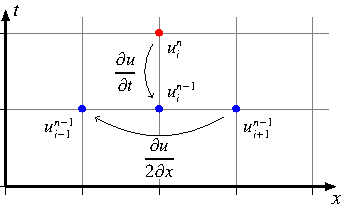
\includegraphics[height=.4\textwidth]{papers/burgers/BurgersEquation/tikz/linear4/linear4.pdf}
		\caption{Explizite Leap-Frog Methode}
		\label{burgers:fig:Linear4}
		\end{figure}

	Wiederum kann die Gleichung
	\begin{equation}
	\frac {\partial u}{\partial t}+u{\frac {\partial u}{\partial x}} \cong \frac{u_{i}^{n}-u_{i}^{n-1}}{\Delta t}+ u_{i}^{n}\, \frac{u_{i+1}^{n-1}-u_{i-1}^{n-1}}{2\,\Delta x}=0
	\end{equation}
	diskretisiert und nach dem gesuchten Punkt


	\begin{equation}
	u_{i}^{n} = \frac{2 \Delta{x}\, u^{n-1}_{i}\,}{\Delta{t}\, u^{n-1}_{i+1}\, - \Delta{t}\, u^{n-1}_{i-1}\, + 2 \Delta{x}\,}
	\end{equation}
 aufgel\"ost werden.

\medskip

	Wie bereits in den gezeigten Varianten kann f\"ur die Multiplikation der Punkt $u_{i}^{n-1}$ verwendet werden (\autoref{burgers:fig:Linear3}).
	Die Diskretisierung \"andert sich zu

	\begin{figure}
	\centering
	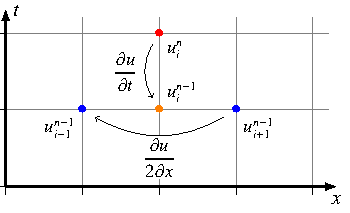
\includegraphics[height=.4\textwidth]{papers/burgers/BurgersEquation/tikz/linear3/linear3.pdf}
	\caption{Explizite Leap-Frog Methode mit  $u_{i}^{n-1}$ f\"ur die Multiplikation}
	\label{burgers:fig:Linear3}
	\end{figure}



	\begin{equation}
		\frac {\partial u}{\partial t}+u{\frac {\partial u}{\partial x}} \cong \frac{u_{i}^{n}-u_{i}^{n-1}}{\Delta t}+ u_{i}^{n-1}\, \frac{u_{i+1}^{n-1}-u_{i-1}^{n-1}}{2\,\Delta x}=0
		\label{burgers:eq_ex_lf1}
	\end{equation}
 	und die L\"osung kann berechnet werden als
	\begin{equation}
	 u_{i}^{n} = \frac{u^{n-1}_{i}\, \left(- \Delta{t}\, u^{n-1}_{i+1}\, + \Delta{t}\, u^{n-1}_{i-1}\, + 2 \Delta{x}\,\right)}{2 \Delta{x}\,}.
		\label{burgers:eq_ex_sol_lf1}
	\end{equation}



\subsubsection{Stabilit\"atskriterium Leap-Frog Verfahren}
	Mit der Einf\"uhrung des Leap-Frog Verfahrens wurde eine unerw\"unschte Instabilit\"at in das System gebracht.
	Die Problematik ist, dass im Raum über zwei Raumschritte abgetastet wird.
	Dabei kann schon in einem Abtastschritt eine Änderung vorkommen.
	Von einer technischer Blickrichtung kann von einer Verletzung des Nyquist-Shannon-Abtasttheorems gesprochen werden.
	Die Abtastrate beträgt nicht das Doppelte der höchsten Frequenz im System.

	\medskip

	Die erw\"ahnte Instabilit\"at im Abschnitt \ref{burgers:sec:nwp}, auf die Richardson gestossen ist, ist die hier beschriebe.
\index{Richardson, Lewis Fry}%
	Ein analytisches Beispiel aus der Biografie von Richardson \cite{burgers:lynch_2014} mit der Differentialgleichung der Reibung.

	\begin{equation}
		\frac{dQ}{dt} = - \kappa Q, \,\,\,\,\, \text{wobei} \, \,\,\,\,\,\, Q=Q^0 \,\,\,\,\,\,\, \text{bei} \,\,\,\,\,\,\,\, t=0.
	\end{equation}
	Mit dem expliziten Verfahren w\"urde die Diskretisierung wie folgt aussehen:
	\begin{equation}
		\frac{Q^{n+1}-Q^n}{\Delta t} = - \kappa Q^n.
	\end{equation}
	Die L\"osung
		\begin{equation}
			Q^n = Q^0(1-\kappa \Delta t)^n
		\end{equation}
	ist eine monoton fallende geometrische Reihe, falls $|\kappa \Delta t| <1$.

	\medskip
	Wird nun das Leap-Frog Verfahren angewendet \"andert sich die Diskretisierung zu
	\begin{equation}
		\frac{Q^{n+1}-Q^{n-1}}{2 \Delta t} = - \kappa Q^n.
	\end{equation}
	Die Gleichung kann weiter nach
	\begin{equation}
		-\frac{Q^{n+1}-Q^{n-1}}{\kappa 2 \Delta t} = Q^n
	\end{equation}
	aufgelöst werden.
	Die Lösung dieser linearen Differentialgleichung kann mit einem Potenzansatz der Form
		\begin{equation}
			Q^n = Q^0\xi ^n.
			\label{burgers:eq_cm}
		\end{equation}
	gefunden werden.
	Dies ist wiederum eine monoton fallende L\"osung gegen Null, wenn $0 < \xi < 1$.
	Setzen wir f\"ur $Q^n = \xi$, $Q^{n+1} = \xi^2$ und $Q^{n-1} = \xi^0$,
	erhält man
	\begin{equation}
		\frac{\xi^2 -1}{2\Delta t} =  -\kappa \xi.
	\end{equation}
    Diese quadratische Gleichung kann mit den folgenden Schritten aufgelöst werden:
\begin{subequations}
    \begin{align}
            \xi^2 + (\kappa 2 \Delta t) \xi  -1 &= 0 \\
            \xi &= \frac{- \kappa 2 \Delta t \pm \sqrt{(\kappa 2 \Delta t)^2 + 4}}{2}\\
            \xi_+ &= - \kappa\Delta t + \sqrt{\kappa^2 \Delta t^2 + 1}\\
            \xi_- &= - \kappa\Delta t - \sqrt{\kappa^2 \Delta t^2 + 1}.
        \end{align}
    \end{subequations}
	Man sieht, dass $|\xi_+| < 1$ und somit eine abfallende, gegen Null gehende L\"osung entsteht.
	Allerdings ist 	$|\xi_-| > 1$ und damit w\"achst die zu $\xi_-$ gehörige Lösung ohne Limit mit $n$.
	Dieser Anteil wird der  \textit{computational mode} genannt und entsteht bei der Verwendung des expliziten Leap-Frog Verfahren.
\index{computational mode}%
	In \autoref{burgers:fig:cmr} kann der Verlauf der Lösungen für $\xi$ betrachted werden.
	\begin{figure}
	\centering
	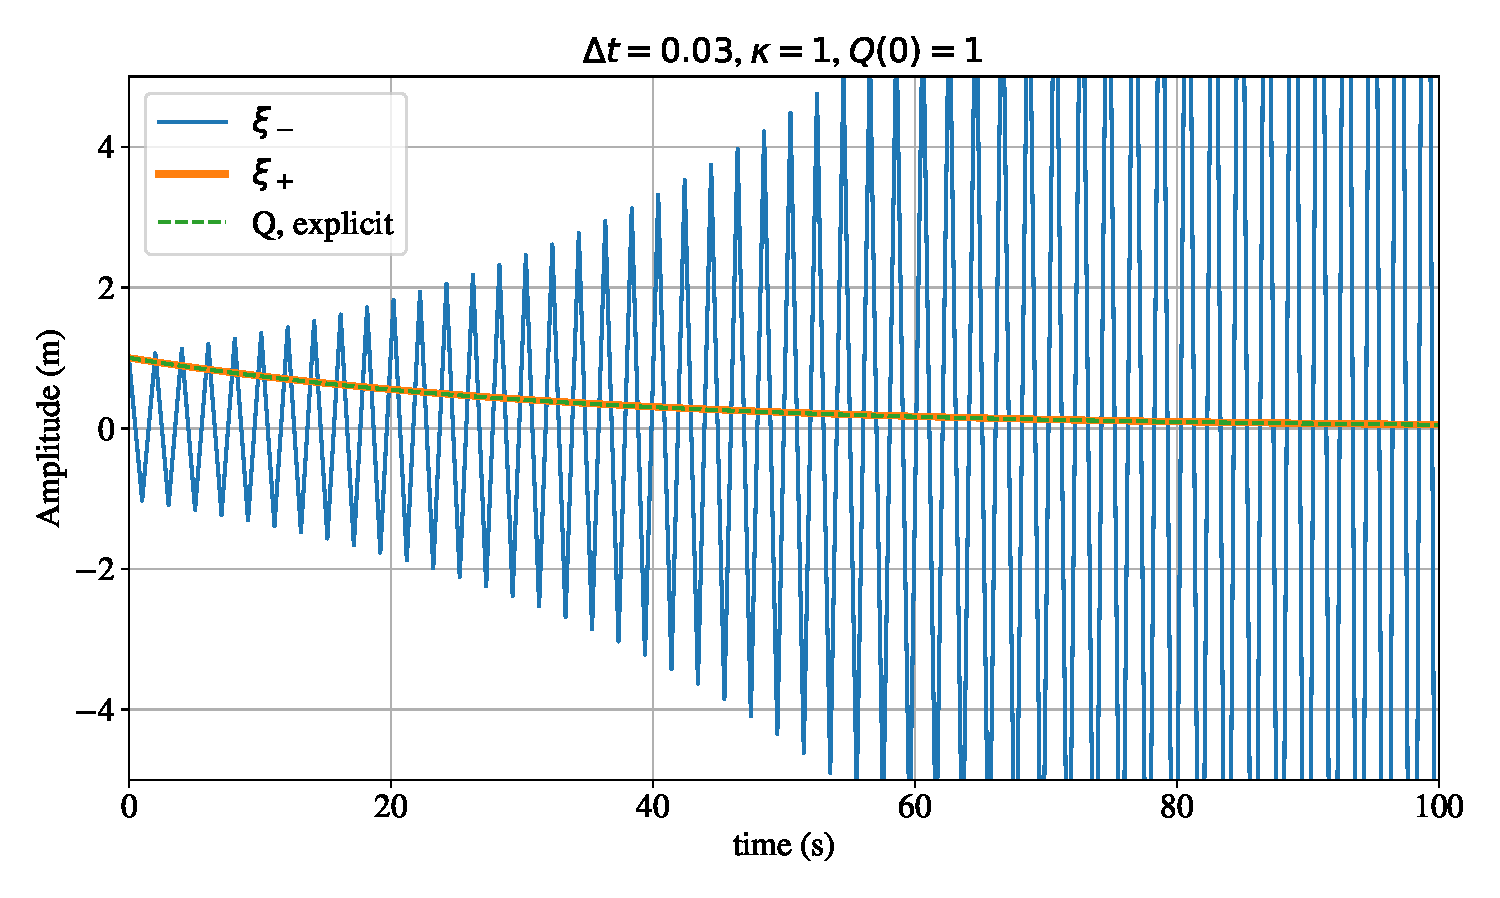
\includegraphics[width=1\textwidth]{papers/burgers/BurgersEquation/comp_mode.pdf}
	\caption{Computational mode für die Differentialgleichung der Reibung}
	\label{burgers:fig:cmr}
	\end{figure}

	In \autoref{burgers:fig:cm1} kann diese Instabilit\"at mit der Gleichung von Burgers beobachtet werden.
	Mit fortschreitender Zeit w\"urde die L\"osung gegen $\infty$ gehen.


  \begin{figure}
	\centering
	\includegraphics[width=.49\textwidth]{papers/burgers/BurgersEquation/images/Leap_Frog_front.pdf}
	\includegraphics[width=.49\textwidth]{papers/burgers/BurgersEquation/images/Leap_Frog_top.pdf}
	\caption{Computational mode für die Burgers Gleichung}
	\label{burgers:fig:cm1}
	\end{figure}

	\paragraph{Unterdrückung des Computational Mode}
	\label{burgers:sec:cm}

	Dieser hochfrequente Fehler kann mittels eines digitalen Tiefpassfilters eliminiert werden.
\index{Tiefpassfilter}
	Das sogenannte Robert-Asselin-Time-Filter \cite{burgers:time_filter} kann hierf\"ur eingesetzt werden.
\index{Robert-Asselin-Time-Filter}%
	Das Filter
		\begin{equation}
			\hat{u}(t_n,x_i) = u(t_n,x_i)+ \frac{\alpha}{2} [ \, u(t_n,x_{i-1}) - 2u(t_n,x_i)+u(t_n,x_{i+1}) ] \,
		\end{equation}
	wird in dieser Anwendung allerdings nicht auf die Zeit, sondern auf die Raum-Dom\"ane angewendet.
	Mit dem D\"ampfungsfaktor $\alpha$ kann das Filter auf die Applikation angepasst werden.

\subsection{Implizit}
\index{implizites Verfahren}%
	Beim impliziten Verfahren werden Datenpunkte der gleichen Zeitebene wie der gesuchte Punkt $u_{i}^{n}$ verwendet.


\subsubsection{Quadratisch}
     \begin{figure}
	\centering
	\includegraphics[height=.4\textwidth]{papers/burgers/BurgersEquation/tikz/quadratic/quadratic.pdf}
	\caption{Implizite quadratische Methode}
	\label{burgers:fig:quadratic}
	\end{figure}

	Die direkteste Art der Diskretisierung, \autoref{burgers:fig:quadratic}, kann wie folgt beschrieben werden.
	Da der Punkt $u_{i}^{n}$ f\"ur die Multiplikation verwendet wird, entsteht
	\begin{equation}
	\frac {\partial u}{\partial t}+u{\frac {\partial u}{\partial x}} \cong \frac{u_{i}^{n}-u_{i}^{n-1}}{\Delta t}+ u_{i}^{n}\, \frac{u_{i}^{n}-u_{i-1}^{n}}{\Delta x}=0.
	\end{equation}
	Die beiden L\"osungen dieser quadratischen Gleichung sind

	\begin{equation}
	  u_{i}^{n} =
	     \dfrac{\Delta{t}\, u^{n}_{i-1}\, - \Delta{x}\, \pm \sqrt{\Delta{t}\,^{2} (u^{n}_{i-1})^{2} + 4 \Delta{t}\, \Delta{x}\, u^{n-1}_{i}\, - 2 \Delta{t}\, \Delta{x}\, u^{n}_{i-1}\, + \Delta{x}\,^{2}}}{2 \Delta{t}},
	\end{equation}
	dabei f\"uhrt der negative Teil der L\"osung zu einer Instabilität.


	\subsubsection{Linear}
	\label{burgers:sec:imp_lin}
	     \begin{figure}
		\centering
		\includegraphics[height=.4\textwidth]{papers/burgers/BurgersEquation/tikz/linear5/linear5.pdf}
		\caption{Implizite lineare Methode}
		\label{burgers:fig:linear5}
		\end{figure}

		Wird wie gewohnt der Wert  $u_{i}^{n-1}$ f\"ur die Multiplikation verwendet, entsteht eine simplere lineare Gleichung
	    \begin{equation}
		\frac {\partial u}{\partial t}+u{\frac {\partial u}{\partial x}} \cong \frac{u_{i}^{n}-u_{i}^{n-1}}{\Delta t}+ u_{i}^{n-1}\, \frac{u_{i}^{n}-u_{i-1}^{n}}{\Delta x}=0,
		\label{burgers:eq:imp_lin}
		\end{equation}
		die in \autoref{burgers:fig:linear5} dargestellt ist.
	    Die L\"osung kann mit
	    \begin{equation}
		 u_{i}^{n} = \frac{u^{n-1}_{i}\, \left(\Delta{t}\, u^{n}_{i-1}\, + \Delta{x}\,\right)}{\Delta{t}\, u^{n-1}_{i}\, + \Delta{x}\,}
		 \label{burgers:eq:imp_lin_sol}
		\end{equation}
	    gefunden werden.

	\subsubsection{Leap-Frog Verfahren}

		Mit dem impliziten Leap-Frog Verfahren (\autoref{burgers:fig:Implicit}) kann f\"ur die Ableitung im Raum der Wert an der korrekten Stelle berechnet werden.
		Nun wird allerdings der Punkt  $u_{i+1}^{n}$ f\"ur die Berechnung verwendet, welcher bei der Berechnung des Punktes  $u_{i}^{n}$ noch unbekannt ist.
		Somit entsteht ein lineares Gleichungssystem.

	    \begin{figure}
		\centering
		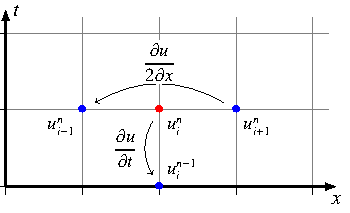
\includegraphics[height=.4\textwidth]{papers/burgers/BurgersEquation/tikz/implicit/implicit.pdf}
		\caption{Implizite leap-frog Methode}
		\label{burgers:fig:Implicit}
	\end{figure}
	Um das lineare Gleichungssystem in gewohnter Notation zu schreiben, werden alle Werte auf der Zeitebene $u^n$ als gesuchte Variablen angenommen.
	Bei Diskretisierung mit dem Leap-Frog Verfahren entsteht
	\begin{equation}
	\frac {\partial u}{\partial t}+u{\frac {\partial u}{\partial x}} \cong \frac{u_{i}^{n}-u_{i}^{n-1}}{\Delta t}+ u_{i}^{n-1}\, \frac{u_{i+1}^{n}-u_{i-1}^{n}}{2\,\Delta x}=0.
	\end{equation}
	Die Gleichung kann nach den Unbekannten
	\begin{equation}
	   -u_{i}^{n-1} \, \Delta t \, u_{i-1}^{n} +  2 \, \Delta x \,  u_{i}^{n} + u_{i}^{n-1} \, \Delta t \, u_{i+1}^{n} =  2 \, \Delta x \, u_{i}^{n-1}
	\end{equation}
	sortiert werden.
	%\begin{subequations}
	%  \begin{align}
	%  \frac{u_{i}^{n+1}-u_{i}^{n}}{dt} &= -u_{i}^{n} \, \frac{u_{i+1}^{n+1} - u_{i-1}^{n+1}}{2 \, dx} \\
	%    u_{i}^{n+1}-u_{i}^{n} &= -u_{i}^{n} \, dt \, \frac{u_{i+1}^{n+1} - u_{i-1}^{n+1}}{2 \, dx}\\
	 %   u_{i}^{n+1} &= -u_{i}^{n} \, dt \, \frac{u_{i+1}^{n+1} - u_{i-1}^{n+1}}{2 \, dx} + u_{i}^{n}\\
	%    2 \, dx \,  u_{i}^{n+1} &= -u_{i}^{n} \, dt \, \left(u_{i+1}^{n+1} - u_{i-1}^{n+1} \right) + 2 \, dx \, u_{i}^{n}\\
	%    2 \, dx \,  u_{i}^{n+1} + u_{i}^{n} \, dt \, u_{i+1}^{n+1} -u_{i}^{n} \, dt \, u_{i-1}^{n+1} & =  2 \, dx \, u_{i}^{n}\\
	%   -u_{i}^{n} \, dt \, u_{i-1}^{n+1} +  2 \, dx \,  u_{i}^{n+1} + u_{i}^{n} \, dt \, u_{i+1}^{n+1} &=  2 \, dx \, u_{i}^{n}
	%  \end{align}
	%\end{subequations}


	%\begin{equation}
	%  u_{i}^{n+1}-u_{i}^{n} = -u_{i}^{n} \, dt \, \frac{u_{i+1}^{n+1} - u_{i-1}^{n+1}}{2 \, dx}
	%\end{equation}
	%\begin{equation}
	%  u_{i}^{n+1} = -u_{i}^{n} \, dt \, \frac{u_{i+1}^{n+1} - u_{i-1}^{n+1}}{2 \, dx} + u_{i}^{n}
	%\end{equation}
	%\begin{equation}
	%2 \, dx \,  u_{i}^{n+1} = -u_{i}^{n} \, dt \, \left(u_{i+1}^{n+1} - u_{i-1}^{n+1} \right) + 2 \, dx \, u_{i}^{n}
	%\end{equation}
	%\begin{equation}
	%  2 \, dx \,  u_{i}^{n+1} + u_{i}^{n} \, dt \, u_{i+1}^{n+1} -u_{i}^{n} \, dt \, u_{i-1}^{n+1} =  2 \, dx \, u_{i}^{n}
	%\end{equation}
	%\begin{equation}
	% -u_{i}^{n} \, dt \, u_{i-1}^{n+1} +  2 \, dx \,  u_{i}^{n+1} + u_{i}^{n} \, dt \, u_{i+1}^{n+1}=  2 \, dx \, u_{i}^{n}
	%end{equation}
	F\"ur die Randpunkte kann das Leap-Frog Verfahren nicht angewendet werden.
	Nachfolgend wurde f\"ur diese Punkte das Verfahren in \autoref{burgers:sec:imp_lin} verwendet.

	Das Gleichungssystem kann in Matrix-Notation umgeschrieben werden als
	\begin{equation}
	\left[{\begin{matrix}
	{dx- u_{1}^{n-1}\, \Delta t}&{ u_{1}^{n-1} \, \Delta t}&{0}&{\dots}&{0}\\[5pt]
	{-u_{2}^{n-1} \, \Delta t}&{ 2 \, \Delta x}&{ u_{2}^{n-1} \, \Delta t}&{\dots}&{0}\\[5pt]
	{0}&{-u_{3}^{n-1} \, \Delta t}&{ 2 \, \Delta x}&\ddots &{0}\\[5pt]
	{0}&{0}&\ddots &\ddots &{ u_{M-1}^{n-1} \, \Delta t}\\[5pt]
	{0}&{0}&{\dots}&{-u_{M}^{n-1} \, \Delta t}&{\Delta x + u_{M}^{n-1}\, \Delta t}
	\end{matrix}}
	\right]\left[{\begin{matrix}
	{ u_{1}^{n}}\\[5pt]
	{ u_{2}^{n}}\\[5pt]
	{ u_{3}^{n}}\\[5pt]
	\vdots \\[5pt]
	{ u_{M}^{n}}
	\end{matrix}}\right]
	=\left[{\begin{matrix}
	{\Delta x \, u_{1}^{n-1}}\\[5pt]
	{ 2 \, \Delta  \, u_{2}^{n-1}}\\[5pt]
	{ 2 \, \Delta x \, u_{3}^{n-1}}\\[5pt]
	\vdots \\[5pt]
	{\Delta x \, u_{M}^{n-1}}
	\end{matrix}}\right].
	  \end{equation}
	Matrizen mit dieser Anordnung werden tridiagonale Matrizen genannt.
\index{tridiagonal}%
	Die Gleichungen haben die allgemeine Form
	  \begin{equation}
	    a_{i}x_{{i-1}}+b_{i}x_{i}+c_{i}x_{{i+1}}=d_{i}
	  \end{equation}
	oder in Matrixform
	  \begin{equation}
	    \begin{bmatrix}{b_{1}}&{c_{1}}&{}&{}&{0}\\
	      {a_{2}}&{b_{2}}&{c_{2}}&{}&{}\\
	      {}&{a_{3}}&{b_{3}}&\ddots &{}\\
	      {}&{}&\ddots &\ddots &{c_{n-1}}\\
	      {0}&{}&{}&{a_{n}}&{b_{n}}\\
	      \end{bmatrix}
	      \begin{bmatrix}{x_{1}}\\
	      {x_{2}}\\{x_{3}}\\\vdots \\
	      {x_{n}}\\
	      \end{bmatrix}
	      =
	      \begin{bmatrix}{d_{1}}\\
	      {d_{2}}\\{d_{3}}\\
	      \vdots \\{d_{n}}\\
	    \end{bmatrix}
	  \end{equation}
	   und k\"onnen mit dem Thomas-Algorithmus \autoref{TDMA} \cite{burgers:thomas} mit der Geschwindigkeit $O(n)$ gel\"ost werden.
\index{Thomas-Algorithmus}%
	   Mehr zum Algorithmus im Abschnitt \ref{buch:subsection:thomasalgorithmus}.

	\begin{algorithm}\caption{Tridiagonal matrix algorithm (Thomas algorithm)}\label{TDMA}
	  \setlength{\lineskip}{7pt}
	  \begin{algorithmic}[1]
	    \Function{Thomas}{$\textbf{a}, \textbf{b}, \textbf{c}, \textbf{d}$}
	      \Comment{Vectors}
	      \State $\hat c_1 \gets$ $ \dfrac{c_1}{b_1}$
	      \State $\hat d_1 \gets \dfrac{d_1}{b_1}$
	      \For{$i = 2,3,\dots,n-1$}
	      \Comment{Forward sweep}
	        \State $\hat c_i \gets \dfrac{c_i}{b_i-a_i \, \hat c_{i-1}}$
	      \EndFor
		  \For{$i = 2,3,\dots,n$}
	      \Comment{Forward sweep}
	        \State $\hat d_i \gets \dfrac{d_i - a_i \, \hat d_{i-1}}{b_i-a_i \, \hat c_{i-1}}$
	      \EndFor
	      \State $x_n \gets \hat d_n$
	      \For{$i = n-1,n-2,\dots,1$}
	      \Comment{Backwards substitution}
	        \State $x_i \gets \hat d_i - \hat c_i \, x_{i+1}$
	      \EndFor
	      \State \textbf{return} $\textbf{x}$
	    \EndFunction
	  \end{algorithmic}
	\end{algorithm}

	\subsubsection{Stabilit\"atskriterium Implizite Verfahren}

	Eine Instabilit\"at wie in den expliziten Verfahren konnte nicht beobachtet werden.
	All gezeigten Varianten k\"onnen als stabil betrachtet werden.
	Mehr dazu im Abschnitt \ref{pde:subsection:stabilitaet}
